% importa variabili globali
% definizione variabili globali
\def\GRUPPO {\textit{DazzleWorks}}

\def\PROGETTO {\textbf{Premi}}

\def\COMMITTENTE {Prof. Vardanega Tullio, \\ & Dr. Cardin Riccardo}

\def\EMAIL {dazzleworksgroup@gmail.com}

\def\LOGO {../../template/img/logo.png}

\def\INTESTAZIONE {../../template/img/intestazione.png}
\def\PIEDIPAGINA {../../template/img/piedipagina.png}

\def\G {{\small $_G$}}



% definizione variabili locali
\def\DOCUMENTO{Piano di Qualifica}
\def\VERSIONE{2.0.0}

\def\REDATTORE {Agostinetto Matteo \\ & Crespan Emanuele}
\def\VERIFICATORE {Ros Fabio}
\def\RESPONSABILE {Carraro Nicola}

\def\USO {Esterno}

\def\DISTRIBUZIONE {\GRUPPO{}\\ & \COMMITTENTE{}\\ & \PROPONENTE{}\\}

\def\DESCRIZIONE {Documento riguardante le strategie di verifica e validazione adottate dal gruppo \GRUPPO\ necessarie ad assicurare i requisiti qualitativi nello svolgimento del progetto \PROGETTO.}


% abilita (true) / disabilita (false) indice, lista tabelle, lista figure
\def\INDICE	{true}
\def\TABELLE {true}
\def\FIGURE {true}


% importa struttura
\documentclass[a4paper]{article}

% ----- definizioni -----
\def\TITLE		{\mbox{\GRUPPO}}
\def\SUBTITLE	{\SIGLA, \PROGETTO}


% ----- nuovi comandi -----
% fornisce il caption per riferirsi ad una particolare sezione
\newcommand{\numref}[1]{\textsf{\textsl{``\nameref{#1}'' (\ref{#1})}}}


% ----- package -----
\usepackage[T1]{fontenc}   % codifica dei font in uscita
\usepackage[utf8x]{inputenc}   % lettere accentate da tastiera
\usepackage[italian]{babel}   % lingua principale del documento
\usepackage[a4paper, top= 3cm, bottom= 3cm, left= 3cm, right= 3cm, bindingoffset= 5mm]{geometry} % impostazione margini

\usepackage{amssymb} %

\usepackage{booktabs} % comandi aggiuntivi per le tabelle

\usepackage{calc} % espressioni aritmetiche
\usepackage{caption} % descrizione figure, ecc
\usepackage{chapterbib} % inclusione delle bibliografie

\usepackage{datatool} % manipolazione dati
\usepackage{dcolumn} % array in tabular

\usepackage{epstopdf} % conversione eps--> pdf
\usepackage{enumitem} % personalizzazione liste
\usepackage{eurosym} % simbolo euro

\usepackage{fancyhdr}   %personalizzazione dello stile
\usepackage{float} % definizione di oggetti floating (es. figure, tabelle)
\usepackage[bottom]{footmisc} % personalizzazione note

\usepackage[toc]{glossaries}	% glossario
\usepackage{graphicx, subfigure} % pacchetto grafica testo
\usepackage{grffile} % estende gestione filename graphic

\usepackage[colorlinks=true, urlcolor=blue, citecolor=black, linkcolor=black, hyperindex, breaklinks]{hyperref} % gestione dei link

\usepackage{ifthen}	% costrutto ifthenelse

% \usepackage{listings} % inserimento pezzi di codice
\usepackage{longtable} % tabelle su più pagine

\usepackage{pgf} % grafica postscript e PDF
\usepackage{pgfplots}	% composizione di grafici
\pgfplotsset{/pgf/number format/use comma, compat=newest}	% opzioni per i grafici

\usepackage{multirow} % span multiriga

\usepackage{tabularx, array} % crea paragrafi a colonne
\usepackage{titlesec} % personalizzazione titoli
\usepackage{tikz} % gestione delle formule
\usepackage{totpages} % conta numero pagine

\usepackage{soul} % gestione letterspacing
\usepackage{subfigure} % gestione delle sottofigure

\usepackage{verbatim} % inserimento testo verbatim, non interpretato

\usepackage{wallpaper} % gestione background

\usepackage{xspace} % spazi automatici per le macro


% ----- posizione etichette -----
\captionsetup{tableposition=top, figureposition=bottom, font=small}


% ----- glossario -----
\loadglsentries{../../glossario/glossario.tex}
\renewcommand*{\glssymbolsgroupname}{Simboli}


% ----- stile pagina -----
\pagestyle{fancy}

	% header
	\fancypagestyle {firststyle} {	% definizione stile "firststyle"
		\fancyhf{}
	}

	% indentazione paragrafo
	%\setlength{\parindent} {0pt}
	\setlength{\headheight} {25pt}

	% intestazione
	\lhead{}
	\rhead{\nouppercase{\leftmark}}
	\renewcommand{\headrulewidth}{0pt}  % no linea sotto intestazione

	% piè di pagina
	\lfoot{\footnotesize{{\DOCUMENTO} \\ {\VERSIONE}}}
	\cfoot{}
	\rfoot{\thepage}
	\renewcommand{\footrulewidth}{0pt}   % no linea sopra piè di pagina


% ----- inizio documento -----
% ----- prima pagina -----
\begin{document}
\thispagestyle{firststyle}

\begin{center}

%   \vspace{7cm}
	\textbf{{\fontsize{40pt}{41pt}\selectfont \PROGETTO}} \\
	\rule{8cm}{3pt}
   
   \vspace{4cm}
   \includegraphics[height= 4cm] {\LOGO}
   
	\vspace{1cm}
   {\fontsize{30pt}{31pt}\selectfont \textbf{\GRUPPO}}
	
	\vspace{5cm}
	{\fontsize{18pt}{24pt}\selectfont \textbf{\DOCUMENTO}}
	
%	\vspace{1cm}
	\begin{center}
		\begin{tabular}{r|l}
				\textbf{Versione} & \VERSIONE \\
				\textbf{Redattori} & \REDATTORE \\
				\textbf{Verificatori} & \VERIFICATORE \\
				\textbf{Responsabili} & \RESPONSABILE \\
				\textbf{Uso} & \USO \\
				\textbf{Lista di distribuzione} & \DISTRIBUZIONE
		\end{tabular}
	\end{center}

	\vspace{1cm}
	\textbf{\DESCRIZIONE}

\end{center}


\newpage

% ----- pagine successive -----
\ULCornerWallPaper{1}{\INTESTAZIONE}
\LLCornerWallPaper{1}{\PIEDIPAGINA}

%\thispagestyle{empty}

\newpage

% diario delle modifiche


% numerazione pagine indici
\pagenumbering{Roman}


\newpage
\section*{Diario delle modifiche}

\begin{table}[h]
\centering
\begin{tabular}{|p{0.3\textwidth}|c|c|c|c|}
	\toprule
		\textbf{Modifiche} & \textbf{Autore} & \textbf{Ruolo} & \textbf{Data} & \textbf{Ruolo} \\
	\midrule
	\midrule
		\textit{Approvazione documento} & Agostinetto Matteo & \textit{Responsabile di Progetto} & 2015-04-09 & v1.0.0 \\
	\midrule
		\textit{Eseguita verifica documento} & Burlin Valerio & \textit{Verificatore} & 2015-04-08 & v0.3.0 \\
	\midrule
		\textit{Modifica sezione Resoconto Attività di Verifica sulla base delle segnalazioni del verificatore} & Suierica Bogdan & \textit{Verificatore Capo} & 2015-04-08 & v0.2.1 \\
	\midrule
		\textit{Eseguita verifica documento} & Burlin Valerio & \textit{Verificatore} & 2015-04-07 & v0.2.0 \\
	\midrule
		\textit{Inserimento sezione Resoconto Attività di Verifica} & Suierica Bogdan & \textit{Verificatore Capo} & 2015-04-06 & v0.1.2 \\
	\midrule
		\textit{Modifica sezioni Visione Generale della Strategia di Verifica e Gestione Amministrativa della Revisione sulla base delle segnalazioni del verificatore} & Bogdan Suierica & \textit{Verificatore Capo} & 2015-03-20 & v0.1.1 \\
	\midrule
		\textit{Eseguita verifica documento} & Burlin Valerio & \textit{Verificatore} & 2015-03-17 & v0.1.0 \\
    \midrule
	    \textit{Completamento sezione Visione Generale della Strategia di Verifica} & Suierica Bogdan & \textit{Verificatore Capo} & 2015-03-16 & v0.0.6 \\
	\midrule
		\textit{Completamento appendice Standard di Qualità} & Crespan Emanuele & \textit{Amministratore di Progetto} & 2015-03-16 & v0.0.5 \\
	\midrule
		\textit{Completamento sezione Gestione Amministrativa della Revisione} & Crespan Emanuele & \textit{Amministratore di Progetto} & 2015-03-15 & v0.0.4 \\
	\midrule
		\textit{Completamento sezione Introduzione ed inizio stesura sezione Visione Generale della Strategia di Verifica} & Suierica Bogdan  & \textit{Verificatore Capo} & 2015-03-12 & v0.0.3 \\
	\midrule
		\textit{Inizio stesura sezione Gestione Amministrativa della Revisione} & Crespan Emanuele & \textit{Amministratore di Progetto} & 2015-03-09 & v0.0.2 \\	                         
	\midrule
		\textit{Inizio stesura sezione Introduzione e appendice Standard di Qualità} & Suierica Bogdan & \textit{Verificatore Capo} & 2015-03-09 & v0.0.1 \\
	\bottomrule
\end{tabular}	
\end{table}

\newpage

% importa indici
% definizione indice
\ifthenelse{\equal{\INDICE}{true}}
	{\tableofcontents \newpage}{}

% definizione lista tabelle
%\ifthenelse{\equal{\TABELLE}{true}} 
%	{\listoftables \newpage}{}

% definizione lista figure
\ifthenelse{\equal{\FIGURE}{true}}
	{\listoffigures \newpage}{}


% numerazione pagine
\pagenumbering{arabic}

	% formato visualizzazione
	\rfoot{\thepage ~di~\pageref{TotPages}}


% separatore
\iffalse
	AOjvdYTJD7mcIIYItfsNiYPbmTTogRSP9hrrb2XPE1laMyQ9NHrPgTCTxnW0eV1YcM3Wqh7t5qThjczeXWq3O5FJ7BBQjoWZovC5
\fi


% importa parti documento

%\section{<nomesezione>}
%\input{sections/<nomefile>.tex}

\section{Introduzione}
\subsection{Scopo del documento}
	Il documento ha lo scopo di definire l'architettura generale e i \gls{design pattern} da utilizzare secondo i quali verrà sviluppato il software del progetto Premi.

\subsection{Scopo del prodotto}
Lo scopo del progetto è realizzare un software per un sistema di rappresentazione di \gls{slide} sfruttando la tecnologia  \gls{HTML5}. Lo scopo principale è quello di creare un prodotto che sia di qualità comparabile, in prestazioni, funzionalità ed effetti visivi, ai maggiori concorrenti già presenti sul mercato (Prezi, Powerpoint, Keynote, Impress, ...).

\subsection{Glossario}
Per prevenire ed evitare qualsiasi dubbio e per permettere una maggiore chiarezza e comprensione del testo su termini ambigui, abbreviazioni e acronimi utilizzati nei vari documenti, essi sono stati raccolti nel \textit{Glossario v2.0.0} nel quale si possono trovare tutte le informazioni desiderate.
Al fine di rendere subito evidente un termine presente nel \textit{Glossario}, esso verrà marcato con il pedice \G\footnote{Per le istruzioni si rimanda al documento \textit{Norme di Progetto v2.0.0} .}.

\subsection{Riferimenti}

\subsubsection{Normativi}
	\begin{itemize}
		\item \textbf{Analisi dei Requisiti:} \textit{Analisi dei Requisiti v3.0.0};
		\item \textbf{Norme di Progetto:} \textit{Norme di Progetto v2.0.0}.
	\end{itemize}

\subsubsection{Informativi}
	\begin{itemize}
		\item \textbf{Design Patterns, elementi per il riuso di software ad oggetti:} Gamma, Helm, Johnson, Vlissides;
		\item \textbf{SWEBOK v3, Guide to the Software Engineering Body of Knowledge:} IEEE Computer Society;
		\item \textbf{Ingegneria del software} Ian Sommerville, Parte terza: \textit{progettazione};
		\item \textbf{Slide del corso:}
				\begin{itemize}
					\item \textbf{Diagrammi delle classi}: \url{http://www.math.unipd.it/~tullio/IS-1/2014/Dispense/E2a.pdf};
					\item \textbf{Diagrammi dei package}: \url{http://www.math.unipd.it/ ~tullio/IS-1/2014/Dispense/E2b.pdf};
					\item \textbf{Pattern}:
					\begin{itemize}
						\item \textit{Architetturali}
							\begin{itemize}
								\item \url{http://www.math.unipd.it/~tullio/IS-1/2014/Dispense/E9.pdf};
								\item \url{http://www.math.unipd.it/~rcardin/pdf/Design\%20Pattern\%20Architetturali\%20-\%20Model\%20View\%20Controller\_4x4.pdf};
							\end{itemize}
						\item \textit{Strutturali}:
						\begin{itemize}
						\item \url{http://www.math.unipd.it/~tullio/IS-1/2014/Dispense/E6.pdf};
						\end{itemize}
						\item \textit{Creazionali}:
						\begin{itemize}
						\item \url{http://www.math.unipd.it/~tullio/IS-1/2014/Dispense/E7.pdf};
						\end{itemize}
						\item \textit{Comportamentali}:
						\begin{itemize}
						\item \url{http://www.math.unipd.it/~tullio/IS-1/2014/Dispense/E8.pdf};
						\end{itemize}
					\end{itemize}
					\item \textbf{Documentazione di Chart.js}: \url{http://chartjs.org/docs};
					\item \textbf{Documentazione di Angular.js}: \url{https://docs.angularjs.org/guide};
					\item \textbf{Documentazione di Reveal.js}: \url{http://github.com/hakimel/reveal.js};
					\item \textbf{Documentazione di Fabric.js}: \url{http://fabricjs.com};
					\item \textbf{Manuale di MongoDb}: \url{https://docs.mongodb.org/manual};
					\item \textbf{Documentazione di Foundation}: \url{http://foundation.zurb.com/docs};
					\item \textbf{Documentazione di Php}: \url{http://php.net/docs.php}.
				\end{itemize}

	\end{itemize}



\newpage
\section{Visione generale della strategia di verifica}
\subsection{Organizzazione}
L'attività di verifica verrà istanziata per ogni processo attuato. La finalità di ogni attività di verifica è garantire la qualità per ogni processo e prodotto.\\
Il processo di verifica, diverso nelle varie fasi del progetto descritte nel \textit{Piano di Progetto v2.0.0}, sarà il seguente:
\begin{itemize}
	\item \textbf{Analisi:} in questa fase si devono seguire i metodi di verifica, descritti nelle \textit{Norme di Progetto v2.0.0}, sui documenti prodotti;
	\item \textbf{Analisi di Dettaglio:} in questa fase si devono verificare i processi che hanno portato ad un incremento nel \gls{versionamento} dei documenti, prodotti nella fase precedente, seguendo le procedure descritte nelle \textit{Norme di Progetto v2.0.0};
	\item \textbf{Progettazione architetturale:} in questa fase, oltre a verificare i processi che hanno portato ad un incremento nel \gls{versionamento} dei documenti, si andranno a verificare i prodotti ed i processi attuati per l'attività di progettazione architetturale;
	\item \textbf{Progettazione di Dettaglio e Codifica:} in questa fase, oltre a verificare i processi che hanno portato ad un incremento nel \gls{versionamento} dei documenti, si andrà a verificare che ogni requisito sia rintracciabile da uno dei componenti emersi durante la fase di progettazione;
	\item \textbf{Verifica e Validazione:} in questa fase, oltre a verificare i processi che hanno portato ad un incremento nel \gls{versionamento} dei documenti, verrà effettuato il collaudo del prodotto garantendone la correttezza.
\end{itemize} 

\subsection{Pianificazione strategica e temporale}
Gli obiettivi fissati possono essere raggiunti solamente attraverso una buona pianificazione in base alla quale si dovrà agire. Con l'obiettivo di rispettare le scadenze fissate nel \textit{Piano di Progetto v2.0.0} è fondamentale un'attività di verifica ben organizzata e sistematica, pertanto è essenziale, prima di iniziare qualsiasi attività, capirne la struttura ed i contenuti. È inoltre necessaria un'attenta lettura delle \textit{Norme di Progetto v2.0.0} in cui sono descritte le varie metodologie da seguire per l'individuazione e la correzione degli errori.

\subsection{Responsabile}
Le responsabilità di tutte le attività di verifica e validazione sono a carico del \textit{Responsabile di Progetto} e dei \textit{Verificatori}. Questi ruoli, durante le varie fasi di progetto, saranno ricoperti da diversi componenti del gruppo, come descritto nel \textit{Piano di Progetto v2.0.0}. Per questo motivo è necessario che tutti i componenti del gruppo siano motivati e incoraggiati ad assumersi le responsabilità per il lavoro svolto e per sviluppare nuovi approcci atti al miglioramento della qualità.

\subsection{Risorse necessarie}
Per assicurarsi che gli obiettivi siano raggiunti e monitorare costantemente lo sviluppo è necessario l'utilizzo sia di risorse umane che tecnologiche. I ruoli che hanno una responsabilità maggiore per l'attività di verifica e validazione sono il \textit{Responsabile di Progetto} e il \textit{Verificatore}. Per una descrizione dettagliata dei ruoli e delle loro responsabilità si rimanda alle \textit{Norme di Progetto v2.0.0}. Inoltre nelle \textit{Norme di Progetto v2.0.0} vengono descritte le risorse tecnologiche, ossia gli strumenti hardware e software necessari alle attività di verifica. Affinché il lavoro delle persone implicate venga agevolato, in particolare del \textit{Verificatore}, si sono predisposti numerosi strumenti automatici garantendo un controllo più semplice e corretto.

\subsection{Attività chiave}
\begin{itemize}
	\item \textbf{Garanzia della qualità:} tutte le attività che sono realizzate all'interno di un sistema e che hanno l'obiettivo di perseguire e soddisfare requisiti di qualità di un servizio. Si tratta di misurazione sistematica, di confronto con uno o più standard di monitoraggio dei processi e \gls{feedback} che garantiscono la prevenzione degli errori; attività a fronte delle quali questi ultimi dovrebbero essere eliminati;
	\item \textbf{Pianificazione della qualità del prodotto:} la selezione di procedure standard appropriate per questo sistema, adattandole per uno specifico progetto software;
	\item \textbf{Controllo della qualità:} la definizione dei processi che assicurano che il team  di sviluppo software segua le procedure e gli standard adottati nel progetto.
\end{itemize}
Per garantire la qualità dei processi e per garantire una corretta pianificazione delle attività descritte in precedenza, si è deciso di aderire allo standard ISO/IEC 15504 conosciuto anche come SPICE(Software Process Improvement and Capability Determination)\footnote{Per una descrizione dettagliata si rimanda all'appendice \ref{15504} .}.
	
\subsection{Misure e Metriche}
Per garantire il raggiungimento degli obiettivi è necessario fissare delle metriche sulla base delle quali poter misurare i risultati ottenuti dalle varie attività di verifica. È dunque di fondamentale importanza saper quantificare, attraverso delle metriche stabilite a priori, il processo di verifica. Grazie al ciclo di vita adottato, descritto nel \textit{Piano di Progetto v2.0.0}, le metriche incerte ed approssimate si potranno migliorare in modo incrementale.\\
Ogni metrica avrà due caratteristiche fondamentali:
\begin{itemize}
	\item \textbf{Range di accettazione:} intervallo entro il quale il prodotto si può ritenere soddisfacente;
	\item \textbf{Range ottimale:} valore entro il quale dovrebbe arrivare la misurazione.
\end{itemize}


\subsection{Metriche per i processi}
Per misurare lo stato di avanzamento dei processi si è scelto di utilizzare indici che ne analizzino i costi e
tempi.
\subsubsection{Schedule Variance (SV)}
Lo Schedule Variance è un indicatore di efficacia e serve a controllare se si è in linea, in anticipo o in ritardo rispetto alla pianificazione temporale delle attività nella \gls{baseline}.
Se SV G > 0 significa che il gruppo di lavoro sta producendo con maggior velocità rispetto a quanto pianificato, viceversa se negativo.
Essendo stati inseriti \gls{slack} durante la pianificazione della \gls{baseline} dei processi, il valore di tale indice è inizialmente positivo.
Parametri utilizzati:
\begin{itemize}
	\item \textbf{Range-accettazione}: $\left[  \geq - \: costo \: preventivo \: fase * 5 \% \right]$
	\item \textbf{Range-ottimale}: $\left[\geq 0\right]$.
\end{itemize}
\subsubsection{Budget Variance (BV)}
Il Budget Variance è un indicatore che ha un valore contabile e finanziario e che serve a controllare se alla data corrente si è speso di più o di meno rispetto a quanto pianificato.
Se BV G > 0 significa che l'attuazione del progetto sta consumando il proprio budget con minor velocità rispetto a quanto pianificato, viceversa se negativo.
Parametri utilizzati:
\begin{itemize}
	\item \textbf{Range-accettazione}: $\left[  \geq - \: costo \: preventivo \: fase * 10 \% \right]$
	\item \textbf{Range-ottimale}: $\left[\geq 0\right]$.
\end{itemize}

\subsection{Metriche per la documentazione}
Come metrica per i documenti redatti si è deciso di utilizzare l'indice di leggibilità \gls{Gulpease}. Rispetto ad altri ha il vantaggio di utilizzare la lunghezza delle parole in lettere anziché in sillabe, semplificandone il calcolo automatico. L'indice è tarato sulla lingua italiana e considera due variabili linguistiche: la lunghezza della parola e la lunghezza della frase rispetto al numero delle lettere. \\
\noindent L'indice è calcolato attraverso la seguente formula:\\
\begin{center}
	$89+ \frac{300*\left(numero\:\ delle\:\ frasi \right)-10*\left(numero\:\ delle\:\ lettere\right)}{numero\:\ delle\:\ parole}$
\end{center}
I risultati sono compresi tra 0 e 100, dove 100 indica la leggibilità più alta e 0 la leggibilità più bassa. In generale risulta che i testi con indice:
\begin{itemize}
	\item Inferiore a 80 sono difficili da leggere per chi ha la licenza elementare;
	\item Inferiore a 60 sono difficili da leggere per chi ha la licenza media;
	\item Inferiore a 40 sono difficile da leggere per chi ha il diploma superiore.
\end{itemize}
Basandoci su queste considerazioni è stato scelto di utilizzare:
\begin{itemize}
	\item \textbf{Range di accettazione:} [40 - 100];
	\item \textbf{Range ottimale:} [50 - 100].
\end{itemize}
	
\subsection{Metriche per il software}
Di seguito saranno descritte le metriche che riguardano il software. Data l'inesperienza del gruppo, questa sezione sarà soggetta a modifiche nelle prossime revisioni.
\begin{itemize}
	\item \textbf{Complessità ciclomatica:} misura direttamente il numero di cammini linearmente indipendenti attraverso il grafo di controllo di flusso. Essa viene calcolata utilizzando il grafo di controllo di flusso del programma: i nodi del grafo corrispondono a gruppi indivisibili di istruzioni, mentre gli archi connettono due nodi se il secondo gruppo di istruzioni può essere eseguito immediatamente dopo il primo gruppo. La complessità ciclomatica può, inoltre, essere applicata a singole funzioni, moduli, metodi o classi di un programma.
	\begin{itemize}
		\item \textbf{Range di accettazione:} [1 - 15];
		\item \textbf{Range ottimale:} [1 - 10].
	\end{itemize}
	\item \textbf{Attributi per classe:} un numero elevato di attributi all'interno della classe potrebbe indicare il bisogno di suddividere la classe in più sotto classi.
	\begin{itemize}
		\item \textbf{Range di accettazione:} [0 - 16];
		\item \textbf{Range ottimale:} [3 - 8].
	\end{itemize}
	\item \textbf{Numero di parametri per metodo:} indica il numero di parametri formali di un metodo. Un numero elevato di parametri potrebbe indicare la necessità di ridurre le funzionalità associate a tale metodo.
	\begin{itemize}
		\item \textbf{Range di accettazione:} [0 - 8];
		\item \textbf{Range ottimale:} [0 - 4].
	\end{itemize}
	\item \textbf{Linee di codice per linee di commento:} indica il rapporto tra il numero di linee di commento e il numero di linee di codice. Il codice poco commentato comporta una difficile manutenibilità.
	\begin{itemize}
		\item \textbf{Range di accettazione:} [>20];
		\item \textbf{Range ottimale:} [>30].
	\end{itemize}
	\item \textbf{Numero di livelli di annidamento:} indica il numero di livelli di annidamento dei metodi. Un numero elevato rappresenta un'alta complessità del codice riducendone il livello di astrazione.
	\begin{itemize}
		\item \textbf{Range di accettazione:} [1 - 6];
		\item \textbf{Range ottimale:} [1 - 3].
	\end{itemize}
	\item \textbf{Copertura del codice:} valore che indica la percentuale di codice che viene eseguito durante i test.
	Un valore elevato indica un'alta probabilità che i moduli testati abbiano pochi errori.
	\begin{itemize}
		\item \textbf{Range di accettazione:} [ $\geq$ 40\%];
		\item \textbf{Range ottimale:} [ $\geq$ 60\%].
	\end{itemize}
\end{itemize}



\newpage
\section{Standard di qualità e metriche}
\subsection{Qualità di processo standard ISO/IEC 15504}\label{15504}
Lo standard ISO/IEC 15504 descrive come i processi debbano essere continuamente controllati in modo da rilevare possibili rischi e debolezze che possano impedire il raggiungimento degli scopi prefissati e di individuarne le cause in modo di migliore l'efficienza dei processi. I risultati dei vari controlli devono essere oggettivi, ripetibili e comparabili perché possano essere utilizzati nel miglioramento dei processi.

\noindent Lo standard ISO/IEC 15504, conosciuto anche come SPICE(Software Process Improvement and Capability Determination), prevede per ogni processo un livello di capacità secondo la seguente ripartizione:

\begin{enumerate}[label*=\arabic*]
	\item \textbf{Incomplete process:} il processo non viene eseguito o non riesce a raggiungere i suoi risultati;
	
	\item \textbf{Performed:} il processo eseguito raggiunge i suoi risultati
		\begin{itemize}
			\item \textbf{Process performance attribute:} è la capacità di un processo di raggiungere gli obiettivi trasformando input identificabili in output identificabili.
		\end{itemize}
		
	\item \textbf{Managed process:} il processo viene eseguito in modo controllato in base a obiettivi definiti
		\begin{itemize}
			\item \textbf{Performance management attribute:} è la capacità del processo di elaborare un prodotto coerente con gli obiettivi fissati;
			\item \textbf{Work product management attribute:} è la capacità del processo di elaborare un prodotto documentato, controllato e verificato.
		\end{itemize}
		
		
	\item \textbf{Established process:} il processo viene eseguito basandosi su principi dell'ingegneria del software ed è in grado di raggiungere i risultati fissati
		\begin{itemize}
			\item \textbf{Process definition attribute:} l'esecuzione del processo si basa su standard di processo per raggiungere i propri obiettivi;
			\item \textbf{Process resource attribute:} è la capacità del processo di attingere a risorse tecniche e umane appropriate per essere attuato efficacemente.
		\end{itemize}
		
	\item \textbf{Predictable process:} il processo viene eseguito costantemente entro limiti definiti per raggiungere i risultati attesi
		\begin{itemize}
			\item\textbf{Measurement attribute:} sono gli obiettivi e le misure di prodotto e di processo che vengono usati per garantire il raggiungimento dei traguardi definiti in supporto ai target aziendali;
			\item \textbf{Process control attribute:} il processo viene controllato tramite misure di prodotto e processo per effettuare correzioni migliorative al processo stesso.
		\end{itemize}
		
\item \textbf{Optimizing process:} il processo cambia e si adatta dinamicamente per raggiungere gli obiettivi aziendali
		\begin{itemize}
			\item \textbf{Process change attribute:} sono i cambiamenti strutturali, di gestione e di esecuzione che vengono gestiti in modo controllato per raggiungere i risultati fissati;
			\item \textbf{Continuous improvement attribute:} sono le modifiche al processo che sono identificate e implementate per garantire il miglioramento continuo nella realizzazione degli obiettivi di \gls{business} dell'organizzazione.
		\end{itemize}

\end{enumerate}

\noindent Ogni attributo di processo descritto sopra è misurabile e lo standard predispone 4 livelli diversi:
\begin{itemize}[label={}]
	\item \textbf{N} non posseduto (0\% - 15\%);
	\item \textbf{P} parzialmente posseduto (16\% - 50\%);
	\item \textbf{L} largamente posseduto (51\% - 85\%);
	\item \textbf{F} completamente posseduto (86\% - 100\%).
\end{itemize}

\subsection{Qualità di prodotto standard ISO/IEC 9126} \label{9126}
Con la sigla \textbf{ISO/IEC 9126} s'individua una serie di normative e linee guida preposte a descrivere un modello di qualità del software.
Esso divide i criteri qualitativi in 3 aree diverse:
\begin{itemize}

	\item \textbf{Qualità in uso:} rappresenta il punto di vista dell'utente sul software;
	\item \textbf{Qualità esterna:} misurano i comportamenti del software sulla base dei test, dall'operatività e dall'osservazione durante la sua esecuzione;
	\item \textbf{Qualità interna:} è la qualità del prodotto software vista dall'interno, si riferisce quindi alle caratteristiche d'implementazione quali l'architettura ed i codici sorgenti.
\end{itemize}

\noindent Il modello di qualità dello standard prevede 6 caratteristiche qualitative principali, suddivise in ulteriori sotto caratteristiche, misurabili quantitativamente tramite metriche specifiche.

\begin{figure}[h]
\centering
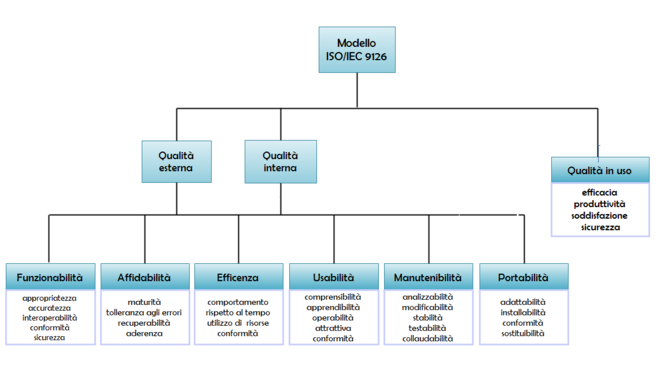
\includegraphics[width=0.7\linewidth]{img/ISO_IEC_9126}
\caption[Rappresentazione globale del modello ISO-IEC 9126]{Rappresentazione globale del modello ISO-IEC 9126}
\label{fig:ISO_IEC_9126}
\end{figure}


\begin{itemize}
\item \textbf{Funzionalità:} è la capacità di un prodotto software di fornire funzioni che soddisfano esigenze stabilite:

\begin{itemize}
	\item \textbf{Idoneità:}  rappresenta la capacità del prodotto software di fornire un appropriato insieme di funzioni per gli specificati compiti e obiettivi prefissati all'utente;
	\item \textbf{Accuratezza:} è la capacità del prodotto software di fornire i risultati concordati;
	\item \textbf{Interoperabilità:} è la capacità del prodotto software di interagire ed operare con uno o più sistemi;
	\item \textbf{Conformità:} è la capacità del prodotto software di aderire a standard, convenzioni e regolamentazioni;
	\item \textbf{Sicurezza:} è la capacità del prodotto software di proteggere informazioni e dati impedendo che persone o sistemi non autorizzati passano accedervi o modificarli.
\end{itemize}

\item \textbf{Affidabilità:} è la capacità del prodotto software di mantenere uno specificato livello di prestazioni:
\begin{itemize}
	\item \textbf{Maturità:} è la capacità di un prodotto software di evitare che si verificano errori o malfunzionamenti;
	\item \textbf{Tolleranza agli errori:} è la capacità di un prodotto software di mantenere un adeguato livello di prestazioni anche nel caso si verifichino errore o malfunzionamenti;
	\item \textbf{Recuperabilità:} è la capacità del prodotto software di ristabilire un adeguato livello di performance e di recuperare i dati interessati in caso di errori;
	\item \textbf{Aderenza:} è la capacità di aderire a standard, regole e convenzioni inerenti all'affidabilità.
\end{itemize}

\item \textbf{Efficienza:} è la capacità di fornire appropriate prestazioni relativamente alla quantità di risorse usate:
\begin{itemize}
	\item \textbf{Comportamento rispetto al tempo:} è la capacità di fornire adeguati tempi di risposta, elaborazione e velocità sotto determinate condizioni;
	\item \textbf{Utilizzo delle risorse:} è la capacità di utilizzo di quantità e tipo di risorse in maniera adeguata;
	\item \textbf{Conformità:} è la capacità di aderire a standard e specifiche sull'efficienza.
\end{itemize}

\item \textbf{Usabilità:} è la capacità del prodotto software di essere appreso e usato dall'utente sotto specifiche condizioni:
\begin{itemize}
	\item \textbf{Comprensibilità:} esprime la facilità di comprensione dei concetti del prodotto;
	\item \textbf{Apprendibilità:} è la capacità di ridurre l'impegno richiesto agli utenti per apprendere l'uso del prodotto;
	\item \textbf{Operabilità:} è la capacità del prodotto software di consentire all'utente di usarlo e controllarlo;
	\item \textbf{Attrattività:} è la capacità del software di essere piacevole per l'utente che ne fa uso;
	\item \textbf{Conformità:} è la capacità del software di aderire a standard o convenzioni relativi l'usabilità.
\end{itemize}
\item \textbf{Manutenibilità:} è la capacità del software di essere modificato, includendo correzioni, miglioramenti o adattamenti:
\begin{itemize}
	\item \textbf{Analizzabilità:} rappresenta la facilità con la quale è possibile analizzare il codice per localizzare un errore;
	\item \textbf{Modificabilità:} è la capacità del prodotto software di permettere l'implementazione di una specificata modifica;
	\item \textbf{Stabilità:} è la capacità del software di evitare effetti inaspettati derivanti da modifiche errate;
	\item \textbf{Testabilità:} è la capacità di essere facilmente testato per validare le modifiche apportate al software.
\end{itemize}

\item \textbf{Portabilità:} è la capacità del software di essere trasportato da un ambiente di lavoro a un altro:
\begin{itemize}
	\item \textbf{Adattabilità:} è la capacità del software di essere adattato per differenti ambienti operativi senza dover applicare modifiche;
	\item \textbf{Installabilità:} è la capacità del software di essere installato in uno specificato ambiente;
	\item \textbf{Conformità:} è la capacità del prodotto software di aderire a standard e convenzioni relative la portabilità;
	\item \textbf{Sostituibilità:} è la capacità di essere utilizzato al posto di un altro software per svolgere gli stessi compiti nello stesso ambiente.
\end{itemize}

\end{itemize}


\subsection{Metriche per i processi}
\label{sezione 3.7}
Per misurare lo stato di avanzamento dei processi si è scelto di utilizzare indici che ne analizzino i costi e
tempi.
\subsubsection{Schedule Variance (SV)}
Lo Schedule Variance è un indicatore di efficacia e serve a controllare se si è in linea, in anticipo o in ritardo rispetto alla pianificazione temporale delle attività nella baseline.
Se SV G > 0 significa che il gruppo di lavoro sta producendo con maggior velocità rispetto a quanto pianificato, viceversa se negativo.
Essendo stati inseriti slack durante la pianificazione della baseline dei processi, il valore di tale indice è inizialmente positivo.
Parametri utilizzati:
\begin{itemize}
	\item \textbf{Range-accettazione}: $\left[  \geq - \: costo \: preventivo \: fase * 5 \% \right]$
	\item \textbf{Range-ottimale}: $\left[\geq 0\right]$.
\end{itemize}
\subsubsection{Budget Variance (BV)}
Il Budget Variance è un indicatore che ha un valore contabile e finanziario e che serve a controllare se alla data corrente si è speso di più o di meno rispetto a quanto pianificato.
Se BV G > 0 significa che l'attuazione del progetto sta consumando il proprio budget con minor velocità rispetto a quanto pianificato, viceversa se negativo.
Parametri utilizzati:
\begin{itemize}
	\item \textbf{Range-accettazione}: $\left[  \geq - \: costo \: preventivo \: fase * 10 \% \right]$
	\item \textbf{Range-ottimale}: $\left[\geq 0\right]$.
\end{itemize}

\subsection{Metriche per la documentazione}
\label{sezione 3.8}
Come metrica per i documenti redatti si è deciso di utilizzare l'indice di leggibilità Gulpease. Rispetto ad altri ha il vantaggio di utilizzare la lunghezza delle parole in lettere anziché in sillabe, semplificandone il calcolo automatico. L'indice è tarato sulla lingua italiana e considera due variabili linguistiche: la lunghezza della parola e la lunghezza della frase rispetto al numero delle lettere. \\
\noindent L'indice è calcolato attraverso la seguente formula:\\
\begin{center}
	$89+ \frac{300*\left(numero\:\ delle\:\ frasi \right)-10*\left(numero\:\ delle\:\ lettere\right)}{numero\:\ delle\:\ parole}$
\end{center}
I risultati sono compresi tra 0 e 100, dove 100 indica la leggibilità più alta e 0 la leggibilità più bassa. In generale risulta che i testi con indice:
\begin{itemize}
	\item Inferiore a 80 sono difficili da leggere per chi ha la licenza elementare;
	\item Inferiore a 60 sono difficili da leggere per chi ha la licenza media;
	\item Inferiore a 40 sono difficile da leggere per chi ha il diploma superiore.
\end{itemize}
Basandoci su queste considerazioni è stato scelto di utilizzare:
\begin{itemize}
	\item \textbf{Range di accettazione:} [40 - 100];
	\item \textbf{Range ottimale:} [50 - 100].
\end{itemize}
	
\subsection{Metriche per il software}
Di seguito saranno descritte le metriche che riguardano il software. Data l'inesperienza del gruppo, questa sezione sarà soggetta a modifiche nelle prossime revisioni.
\begin{itemize}
	\item \textbf{Complessità ciclomatica:} misura direttamente il numero di cammini linearmente indipendenti attraverso il grafo di controllo di flusso. Essa viene calcolata utilizzando il grafo di controllo di flusso del programma: i nodi del grafo corrispondono a gruppi indivisibili di istruzioni, mentre gli archi connettono due nodi se il secondo gruppo di istruzioni può essere eseguito immediatamente dopo il primo gruppo. La complessità ciclomatica può, inoltre, essere applicata a singole funzioni, moduli, metodi o classi di un programma.
	\begin{itemize}
		\item \textbf{Range di accettazione:} [1 - 15];
		\item \textbf{Range ottimale:} [1 - 10].
	\end{itemize}
	\item \textbf{Attributi per classe:} un numero elevato di attributi all'interno della classe potrebbe indicare il bisogno di suddividere la classe in più sotto classi.
	\begin{itemize}
		\item \textbf{Range di accettazione:} [0 - 16];
		\item \textbf{Range ottimale:} [3 - 8].
	\end{itemize}
	\item \textbf{Numero di parametri per metodo:} indica il numero di parametri formali di un metodo. Un numero elevato di parametri potrebbe indicare la necessità di ridurre le funzionalità associate a tale metodo.
	\begin{itemize}
		\item \textbf{Range di accettazione:} [0 - 8];
		\item \textbf{Range ottimale:} [0 - 4].
	\end{itemize}
	\item \textbf{Linee di codice per linee di commento:} indica il rapporto tra il numero di linee di commento e il numero di linee di codice. Il codice poco commentato comporta una difficile manutenibilità.
	\begin{itemize}
		\item \textbf{Range di accettazione:} [>20];
		\item \textbf{Range ottimale:} [>30].
	\end{itemize}
	\item \textbf{Numero di livelli di annidamento:} indica il numero di livelli di annidamento dei metodi. Un numero elevato rappresenta un'alta complessità del codice riducendone il livello di astrazione.
	\begin{itemize}
		\item \textbf{Range di accettazione:} [1 - 6];
		\item \textbf{Range ottimale:} [1 - 3].
	\end{itemize}
	\item \textbf{Copertura del codice:} valore che indica la percentuale di codice che viene eseguito durante i test.
	Un valore elevato indica un'alta probabilità che i moduli testati abbiano pochi errori.
	\begin{itemize}
		\item \textbf{Range di accettazione:} [ $\geq$ 40\%];
		\item \textbf{Range ottimale:} [ $\geq$ 60\%].
	\end{itemize}
\end{itemize}





\newpage
\section{Gestione amministrativa della revisione}
\subsection{Comunicazione e risoluzione di anomalie}
Un'anomalia corrisponde a una mancanza di regolarità e non è conforme a quelle che sono le sue aspettative. Nel corso delle attività di verifica si possono riscontrare anomalie. Esse potranno riguardare:
\begin{itemize}
	\item Violazione delle \textit{Norme di Progettov1.0.0};
	\item Uscita dal range di accettazione da parte di una delle misurazioni;
	\item Distacco rispetto ai requisiti specificati durante l'analisi dei requisiti.
\end{itemize}
Nel caso in cui il verificatore individui un'anomalia dovrà aprire un ticket di segnalazione. Per la gestione completa di questi problemi si rimanda alla consultazione delle \textit{Norme di Progettov1.0.0}.

\subsection{Procedure di controllo di qualità di processo}


\newpage
\section{Pianificazione dei test}
Di seguito verranno descritti tutti i test di validazione, di sistema e di integrazione che sono stati previsti. Si prevede in futuro l'aggiornamento dei test di unit\'a. Per le tempistiche di aggiornamento dei test si faccia riferimento al \textit{Piano di Progetto v2.0.0?}. La dicitura \textbf{N.A.} contenuta nella colonna \textit{Stato} nelle tabelle sottostanti indica che il test non \'e ancora stato applicato in quanto verr\'a applicato solo successivamente, come descritto nel \textit{Piano di Progetto v2.0.0?}.


\subsection{Test di sistema}
In questa sezione vengono descritti i test di sistema che permettono di verificare il comportamento dinamico del sistema nella sua interezza rispetto ai requisiti descritti nell'\textit{Analisi dei Requisiti v2.0.0?}.
I test di sistema descritti sotto, sono quelli che si riferiscono ai requisisti software individuati e quindi meritevoli di un test.

\subsubsection{Descrizione dei test di sistema}
\begin{center}
	\begin{table}[h]
		\begin{tabular}{|l|p{0.7\textwidth}|l|c|}
			\toprule
			
			\textbf{Test} & \textbf{Descrizione} & \textbf{Stato} & \textbf{Requisito} \\
			
			\midrule
			TS1 & Viene verificato che il sistema registri correttamente un utente & N.A. & R[OBB][F]1\\ \midrule
			TS1.1 & Viene verificato che il sistema sia portabile e correttamente visualizzato su desktop, mobile e tablet & N.A & R[OBB][V]-1.1 \\ \midrule
			TS1.6 & Viene verificato che il sistema registri correttamente un utente attraverso un social network & N.A. & R[OPZ][F]1.6\\ \midrule
			TS2 & Viene verificato che il sistema autentichi correttamente un utente & N.A. & R[OBB][F]2\\  \midrule
			TS3	& Viene verificato che il sistema permetta di effettuare una ricerca di un progetto con le modalità implementate & N.A. & R[OBB][F]3\\ \midrule
			TS4	& Viene verificato che il sistema apra un progetto & N.A. & R[OBB][F]4\\ \midrule
			TS5 & Viene verificato che il sistema generi il PDF del progetto & N.A. & R[OBB][F]5\\ \midrule
			TS6 & Viene verificato che il sistema generi un pacchetto stand-alone per la visualizzazione offline & N.A. & R[OBB][F]6\\ \midrule
			TS7 & Viene verificato che il sistema crei un nuovo progetto & N.A. & R[OBB][F]7\\ \midrule
			TS8 & Viene verificato che il sistema apra un progetto precedentemente creato & N.A. & R[OBB][F]8\\ \midrule
			TS9 & Viene verificato che il sistema permetta la modifica del contenuto di una \gls{slide} & N.A. & R[OBB][F]9\\ \midrule
			TS10 & Viene verificato che il sistema crei un'\gls{infografica} & N.A. & R[DES][F]10\\ \midrule
			TS11 & Viene verificato che il sistema permetta di salvare un progetto & N.A. & R[OBB][F]11\\
			
						
			\bottomrule
			
		\end{tabular}
		\caption{Tabella di tracciamento test di sistema/requisiti}
		
	\end{table}
	
\end{center}

\newpage

\subsection{Test di integrazione}
In questa sezione vengono descritti i test di integrazione da usare per testare le componenti descritte nella progettazione ad alto livello, tali test permettono di verificare la corretta implementazione ed il corretto flusso dei dati all'interno del sistema. \'E stato scelto di utilizzare una strategia di integrazione incrementale, che permette lo sviluppo e la verifica delle componenti in parallelo. Unendo infatti le varie componenti per via incrementale, nella maggior parte dei casi, gli errori riscontrati da un test sono da attribuirsi all'ultima parte aggiunta, inoltre con questa strategia è possibile retrocedere e tornare ad uno stato noto e funzionante del sistema. Si \'e deciso di utilizzare il metodo \gls{bottom-up} per integrare prima le componenti con minori dipendenze funzionali e maggiori funzionalit\'a (che corrispondono alle componenti per garantire i requisiti obbligatori) al fine di ottenere il prima possibile una versione funzionante delle parti obbligatorie del sistema. Agendo in questo modo le componenti strettamente legate a parti obbligatorie vengono testate molte volte contribuendo cos\'i ad abbassare il numero di errori in esse contenute. Si procede poi risalendo l'albero delle dipendenze fino ad arrivare alla componente di alto livello alla quale saranno dedicati gli ultimi test.

\begin{figure}[h]
\centering
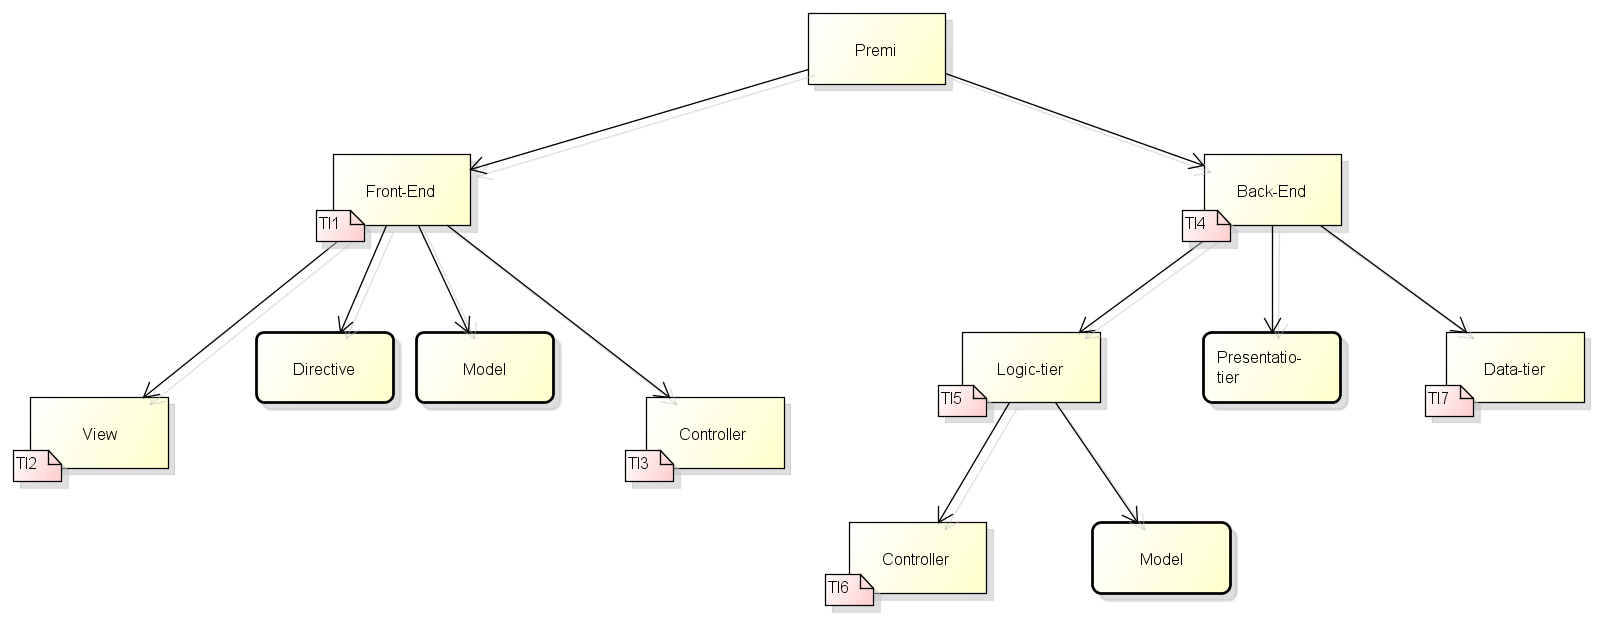
\includegraphics[width=1\linewidth]{img/Integrazione_componenti.png}
\caption[Sequenza d'integrazione delle componenti]{Sequenza d'integrazione delle componenti}
\label{fig:Integrazione_componenti}
\end{figure}

\subsection{Descrizione dei test di integrazione}


\begin{center}
	\begin{table}[h]
		\begin{tabular}{|l|p{0.7\textwidth}|l|c|}
		\toprule
			\textbf{Test} & \textbf{Descrizione} & \textbf{Componente} & \textbf{Stato} \\
			\midrule
			TI1 & Test di controllo finale lato utente & Front-End & N.A\\
			\midrule
			TI2 & Test che verifica la corretta visualizzazione delle interfacce & View & N.A\\
			\midrule
			TI3 & Test che verifica la corretta interazione tra i comandi & Controller & N.A\\
			\midrule
			TI4 & Test che verifica il corretto comportamento tra client e server & Back-End & N.A\\
			\midrule
			TI5 & Test che verifica il corretto funzionamento del server & Logic-tier & N.A\\
			\midrule
			TI6 & Test che verifica la corretta interazione tra i comandidel server & Controller & N.A\\
			\midrule
			TI7 & Test che verifica la correttezza dei dati & Back-End::Data-tier & N.A\\
		\bottomrule
		\end{tabular}
		\caption{Tabella di tracciamento test di integrazione}
	\end{table}
\end{center}

\subsection{Tracciamento componenti–test di integrazione}

\begin{center}
	\begin{table}[h]
		\begin{tabular}{|c|c|}
		\toprule
			\textbf{Componente} & \textbf{Test}\\
			\midrule
			Front-End & TI1\\
			\midrule
			Front-End::View & TI2\\
			\midrule
			Front-End::Controller & TI3\\
			\midrule
			Back-End & TI4\\
			\midrule
			Back-End::Logic-tier & TI5\\
			\midrule
			Back-End::Logic-tier::Controller & TI6\\
			\midrule
			Back-End::Data-tier & TI7\\
		\bottomrule
		\end{tabular}
		\caption{Tabella di tracciamento test di integrazione}
	\end{table}
\end{center}

\newpage

\subsection{Test di validazione}
In questa sezione si descrivono i test di validazione che servono per accertarsi che il prodotto realizzato sia conforme alle aspettative.
Per ogni test vengono descritti i vari passi che un utente deve eseguire per testare i requisiti ad esso associati. Per quanto riguarda il tracciamento test di validazione/requisiti \'e riportato in \textit{Analisi dei Requisiti v2.0.0?}.

\subsection{Test TV1}
L'utente vuole verificare che ci si possa iscrivere. \newline
All'utente \'e richiesto di:
\begin{itemize}
	\item Cliccare il bottone per la registrazione (TV1.1);
	\item Inserire un nome utente univoco (TV1.2);
	\item Inserire una password di almeno 8 caratteri (TV1.3);
	\item Reinserire la password (TV1.4);
	\item Inserire il proprio nome (TV1.5);
	\item Inserire il proprio cognome (TV1.6);
	\item Inserire il proprio indirizzo email (TV1.7);
	\item Confermare i dati inseriti cliccando il bottone "Registrati" (TV1.8);
	\item Controllare di aver ricevuto una email di conferma di avvenuta registrazione (TV1.9).
\end{itemize}

\subsection{Test TV2}
L'utente vuole verificare che ci si possa autenticare. \newline
All'utente \'e richiesto di:
\begin{itemize}
	\item Cliccare il bottone per effettuare il login (TV2.1);
	\item Inserire il proprio nome utente (TV2.2);
	\item Inserire la propria password (TV2.3);
	\item Confermare i dati inseriti cliccando il bottone "Accedi" (TV2.4);
	\item Controllare di poter accedere alla propria pagina personale (TV2.5).
\end{itemize}

\subsection{Test TV3}
L'utente vuole verificare di riuscire a visualizzare i risultati di una ricerca. \newline
All'utente \'e richiesto di:
\begin{itemize}
	\item Effettuare una ricerca usando come chiave un nome utente (TV3.1);
	\item Effettuare una ricerca usando come chiave un titolo di un progetto (TV3.2);
	\item Verificare che compaia la lista dei risultati della ricerca (TV3.3).
\end{itemize}

\subsection{Test TV4}
L'utente vuole verificare di riuscire a visualizzare una presentazione. \newline
All'utente \'e richiesto di:
\begin{itemize}
	\item Aprire una presentazione (TV4.1);
	\item Scegliere l'opzione per la visualizzazione come ascoltatore (TV4.2);
	\item Scegliere l'opzione per la visualizzazione come presentatore (TV4.3);
	\item Verificare che la presentazione sia visualizzata correttamente e che ci si possa muovere liberamente tra le slide (TV4.4).
\end{itemize}

\subsection{Test TV5}
L'utente vuole verificare che il PDF creato sia corretto rispetto al progetto. \newline
All'utente \'e richiesto di:
\begin{itemize}
	\item Aprire un progetto (TV5.1);
	\item Scegliere la funzione di generazione del PDF dall'apposito men\'u (TV5.2);
	\item Verificare che il PDF creato corrisponda al progetto selezionato (TV5.3).
\end{itemize}

\subsection{Test TV6}
L'utente vuole verificare che il progetto esportato sia utilizzabile offline. \newline
All'utente \'e richiesto di:
\begin{itemize}
	\item Aprire un progetto (TV6.1);
	\item Scegliere la funzione di esportazione del progetto dall'apposito men\'u (TV6.2);
	\item Scegliere la posizione in cui salvare il progetto in locale (TV6.3);
	\item Avviare la presentazione in locale del progetto salvato (TV6.4);
	\item Verificare che la presentazione funzioni senza errori e che corrisponda al progetto selezionato (TV6.5);
\end{itemize}

\subsection{Test TV7}
L'utente vuole verificare che sia possibile editare un progetto precedentemente creato. \newline
All'utente \'e richiesto di:
\begin{itemize}
	\item Selezionare un progetto (TV7.1);
	\item Selezionare la slide che si vuole modificare (TV7.2);
	\item Scegliere l'elemento che si desidera modificare o inserirne uno di nuovo (TV7.3)
	\item[] All'utente \'e richiesto di:
	\begin{itemize}
		\item Inserire una nuova slide (TV7.3.1);
		\item Inserire un'immagine (TV7.3.2);
		\item Inserire una casella di testo (TV7.3.3);
		\item Inserire dati \gls{real time} (TV7.3.4);
		\item Inserire una tabella (TV7.3.5);
		\item Inserire un grafico (TV7.3.6);
		\item Selezionare un effetto di transizione (TV7.3.7);
		\item Cambiare la dimensione di un elemento (TV7.3.8);
		\item Cambiare la posizione di un elemento (TV7.3.9);
		\item Ruotare un elemento (TV7.3.10);
		\item Rimuovere un elemento (TV7.3.11);
		\item Modificare una tabella o un grafico (TV7.3.12);
		\item Inserire note/parole chiave (TV7.3.13);
	\end{itemize}
	\item Verificare che le modifiche effettuate siano state applicate al progetto tramite visualizzazione dello stesso (TV7.4).
\end{itemize}

\subsection{Test TV8}
L'utente vuole verificare che si possa salvare un progetto. \newline
All'utente \'e richiesto di:
\begin{itemize}
	\item Creare un nuovo progetto o modificare un progetto già esistente (TV8.1);
	\item Selezionare la funzione di salvataggio (TV8.2);
	\item Dare un nome al progetto (TV8.3);
	\item Verificare che il progetto sia stato salvato, con il nome scelto, nell'apposita sezione riservata ai propri progetti (TV8.4).
\end{itemize}

\subsection{Test TV9}
L'utente vuole verificare che si possa eliminare un progetto. \newline
All'utente \'e richiesto di:
\begin{itemize}
	\item Selezionare il progetto che si vuole eliminare (TV9.1);
	\item Selezionare la funzione di eliminazione del progetto (TV9.2);
	\item Confermare l'eliminazione (TV9.3);
	\item Verificare che il progetto eliminato non sia più presente nell'apposita sezione riservata ai propri progetti (TV9.4).
\end{itemize}

\appendix

\newpage
\section{Riassunto attività di verifica}
\subsection{Riassunto attività di verifica}

Prima di effettuare la consegna dei documenti, allo scadere della milestone, sono state effettuate le attività di verifica dei documenti e dei processi.

I documenti sono stati verificati secondo le procedure descritte nella sezione 2.6.
L`analisi statica dei documenti \'e stata effettuata applicando la tecnica di \textit{walkthrough} per controllare la presenza di errori. Una volta riscontrati gli errori si \'e poi provveduto a segnalarle correggerli. Gli errori pi\'u frequenti sono stati riportati nella sezione lista di controllo presente nelle Norme di Progetti v1.0.0 relativa alla tecnica \textit{inspection}, si \'e poi applicato il ciclo PDCA per migliorare il processo di verifica.
Si \'e poi provveduto ad utilizzare la tecnica \textit{inspection} utilizzando la lista di controllo precedentemente compilata.
Si sono poi calcolate le metriche, descritte nella sezione 2.7.1, per i documenti.
I processi sono stati verificati applicando la procedura descritta nella sezione 2.9.1.

\subsection{Documenti}

Di seguito viene riportata una tabella con gli indici di Gulpease calcolati per ogni documento terminata la fase di verifica.
Ogni documento deve rispettare le metriche descritte nella sezione 2.7.1.\\

\hspace{1cm}

\begin{center}
\begin{tabular}{|c|c|c|}
\hline 
\textbf{Documento} & \textbf{Valore Indice} & \textbf{Risultato} \\ 
\hline
\textit{Norme di Progetto v.1.0.0} & 74 & \textcolor{green}{\textit{Superato}} \\ 
\textit{Studio di Fattibilit\'a v.1.0.0} & 70 & \textcolor{green}{\textit{Superato}} \\ 
\textit{Piano di Progetto v1.0.0} & 69 & \textcolor{green}{\textit{Superato}} \\ 
\textit{Piano di Qualifica v1.0.0} & 70 & \textcolor{green}{\textit{Superato}} \\ 
\textit{Analisi dei Requisiti v1.0.0} & • & \textcolor{green}{\textit{Superato}} \\ 
\textit{Glossario v.1.0.0} & • & \textcolor{green}{\textit{Superato}} \\ 
\hline 
\end{tabular}

\end{center}

\newpage
\section{Dettaglio delle verifiche tramite analisi}
\subsection{Analisi}
\subsubsection{Documenti}
\label{appendice 1}

Di seguito viene riportata una tabella con gli indici di Gulpease calcolati per ogni documento, una volta terminata la fase di verifica. Ogni documento deve rispettare le metriche descritte nella sezione \ref{sezione 3.8} .\\

\hspace{1cm}

\begin{table}[h]
	\begin{tabular}{|c|c|c|}
		\hline 
		\textbf{Documento} & \textbf{Valore Indice} & \textbf{Risultato} \\ 
		\hline
		\textit{Norme di Progetto v1.0.0} & 74 & \textcolor{green}{\textit{Superato}} \\ 
		\textit{Studio di Fattibilità v1.0.0} & 70 & \textcolor{green}{\textit{Superato}} \\ 
		\textit{Piano di Progetto v1.0.0} & 69 & \textcolor{green}{\textit{Superato}} \\ 
		\textit{Piano di Qualifica v10.0} & 70 & \textcolor{green}{\textit{Superato}} \\ 
		\textit{Analisi dei Requisiti v1.0.0} & 79 & \textcolor{green}{\textit{Superato}} \\ 
		\textit{Glossario v1.0.0} & 66 & \textcolor{green}{\textit{Superato}} \\ 
		\hline 
	\end{tabular}
\caption{Indice Gulpease, Analisi}
\end{table}


\subsubsection{Processi}
\label{appendice 2}
\vspace{3mm}

\begin{table}[h]
	\begin{tabular}{|c|c|c|}
		\toprule
			\textbf{Documento} & \textbf{SV\euro} & \textbf{BV\euro} \\ 
		\midrule
		\midrule
			\textit{Norme di Progetto v1.0.0} & -15 & 0 \\ 
			\textit{Studio di Fattibilità v1.0.0} & & -5 \\ 
			\textit{Piano di Progetto v1.0.0} & -15 & -30 \\ 
			\textit{Piano di Qualifica v1.0.0} & -45 & 0 \\ 
			\textit{Analisi dei Requisiti v1.0.0} & 35 & 60 \\ 
			\textit{Glossario v1.0.0} & 0 & 0 \\ 
		\bottomrule
	\end{tabular}
	\caption{Esiti verifica processi, Analisi}
\end{table}

\noindent Complessivamente sono stati registrati:
\begin{itemize}
	\item \textbf{Schedule Variance:} -40 \euro;
	\item \textbf{Budget Variance:} 25 \euro.
\end{itemize}

\noindent Da tali valori si può dedurre che i periodi di slack pianificati non erano sufficienti ad avere una schedule variance positiva, al contrario l'organizzazione del gruppo ha portato ad un costo minore in termini di budget variance. Nonostante lo schedule variance sia negativo, esso rimane comunque al di sopra del minimo accettabile di \euro -142.

\newpage

\subsection{Progettazione Architetturale}
\subsubsection{Documenti}
\label{appendice 3}

Di seguito viene riportata una tabella con gli indici di Gulpease calcolati per ogni documento, una volta terminata la fase di verifica. Ogni documento deve rispettare le metriche descritte nella sezione \ref{sezione 3.8} .\\

\hspace{1cm}

\begin{table}[h]
	\begin{tabular}{|c|c|c|}
		\hline 
		\textbf{Documento} & \textbf{Valore Indice} & \textbf{Risultato} \\ 
		\hline
		\textit{Norme di Progetto v2.0.0} & 74 & \textcolor{green}{\textit{Superato}} \\  
		\textit{Piano di Progetto v2.0.0} & 68 & \textcolor{green}{\textit{Superato}} \\ 
		\textit{Piano di Qualifica v2.0.0} & 71 & \textcolor{green}{\textit{Superato}} \\ 
		\textit{Analisi dei Requisiti v2.0.0} & 79 & \textcolor{green}{\textit{Superato}} \\
		\textit{Specifica Tecnica v1.0.0} & 73 & \textcolor{green}{\textit{Superato}} \\ 
		\textit{Glossario v2.0.0} & 80 & \textcolor{green}{\textit{Superato}} \\ 
		\hline 
\end{tabular}
\caption{Indice Gulpease, Progettazione Architetturale}
\end{table}

\subsubsection{Processi}
\label{appendice 4}
\vspace{3mm}

\begin{table}[h]
	\begin{tabular}{|c|c|c|}
		\toprule
			\textbf{Documento} & \textbf{SV\euro} & \textbf{BV\euro} \\ 
		\midrule
		\midrule
			\textit{Norme di Progetto v2.0.0} & 0 & 0 \\  
			\textit{Piano di Progetto v2.0.0} & 0 & -11 \\ 
			\textit{Piano di Qualifica v2.0.0} & 10 & 0 \\ 
			\textit{Analisi dei Requisiti v2.0.0} & -50 & -25 \\
			\textit{Specifica Tecnica v1.0.0} & 60 & 25 \\ 
			\textit{Glossario v2.0.0} & 0 & 0 \\ 
		\bottomrule
	\end{tabular}
\caption{Esiti verifica processi, Progettazione Architetturale}
\end{table}

\noindent Complessivamente sono stati registrati:
\begin{itemize}
	\item \textbf{Schedule Variance:} 20 \euro;
	\item \textbf{Budget Variance:} -11 \euro.
\end{itemize}

\noindent Da tali valori si può dedurre che i periodi di slack pianificati abbiano aiutato ad avere una schedule variance positiva, al contrario l'inesperienza ad affrontare una progettazione architetturale di un sistema software ha portato ad un costo maggiore in termini di budget variance. Nonostante quest'ultima sia negativa, essa rimane comunque al di sopra del minimo accettabile di \euro -346.

% ...

%\printglossaries

\end{document}
